%!TeX TXS-program:bibliography = txs:///biber
\documentclass[10pt,letterpaper]{article}
\usepackage[latin1]{inputenc}
\usepackage{graphicx}
\usepackage{listings}
\usepackage{hyperref}
\hypersetup{
	colorlinks,
	linkcolor={black},
	citecolor={black},
	urlcolor={blue}
}
\usepackage{float}
\usepackage{acronym}
\usepackage{setspace}
\newcommand{\urlcite}[2]{#2\footnote{\url{#1}}}


\acrodef{DOI}{Digital Object Identifier}
\acrodef{DC}{Dublin Core}
\acrodef{PSID}{Panel Study of Income Dynamics}
\acrodef{ICPSR}{Inter-university Consortium for Political and Social Research}
\acrodef{CMS}{Content Management System}
\acrodef{HCI}{Human-Computer Interaction }
\acrodef{DAS}{Data Accessibility Statement}
\acrodef{FAIR}{Findable, Accessible, Interoperable and Reusable}
\acrodef{FSRDC}{Federal Statistical Research Data Center}
\acrodef{FTI}{Federal Tax Information}
\acrodef{NSO}{National Statistical Organization}
\acrodef{LBD}{Longitudinal Business Database}
\acrodef{PID}{persistent identifier}
\acrodef{AEA}{American Economic Association}
\acrodef{API}{Application Programming Interface}
\acrodef{CSS}{Cascading Style Sheets}
\acrodef{URL}{uniform resource locator}
\acrodef{IDCC}{International Digital Curation Conference}
\acrodef{RDA}{Research Data Alliance}
%\usepackage{natbib}
\usepackage[sorting=nyt,maxnames=10,backend=biber]{biblatex}
\addbibresource{../references-zotero.bib}
\addbibresource{../references.bib}

\author{Lars Vilhuber and Carl Lagoze}
\title{Supplementary Materials}
\begin{document}
	\maketitle
	
\newcommand{\suppDir}{.}
In all use cases, we attempt to identify the three attributes outlined in the main text, using automated mechanisms.

\section{Use Case 1: Public-use information at openICPSR}
In the first case, the researcher has  used public-use data, and identifies a \ac{DOI} to the journal (\url{http://doi.org/10.3886/E100590V1}).  We thus start with the \ac{DOI}, which resolves to the following citation:

\lstset{numbers=left,numberstyle=\tiny,stepnumber=1,basicstyle=\linespread{0.8}\footnotesize}
\begin{quote}
	\it
	McKinney, Kevin L., Green, Andrew S., Vilhuber, Lars, and Abowd, John M. Replication data: Total Error and Variability Measures for QWI and LODES. Ann Arbor, MI: Inter-university Consortium for Political and Social Research [distributor], 2017-12-15. https://doi.org/10.3886/E100590V1
\end{quote}

%We note that this dataset, as all current openICPSR datasets, is licensed under a \href{http://creativecommons.org/licenses/by/4.0/}{Creative Commons Attribution 4.0 International License}. 
\FloatBarrier
\paragraph{DataCite}

We first query the DataCite API (Figure~\ref{fig:case1:datacite}).
\begin{figure}
	\singlespacing
	\lstinputlisting[language=xml,linerange=1-1]{\suppDir/datacite-api-100590.xml}
	\lstinputlisting[language=xml,linerange=9-9,firstnumber=9]{\suppDir/datacite-api-100590.xml}
	\lstinputlisting[language=xml,linerange=10-10,firstnumber=10,basicstyle=\bfseries\footnotesize]{\suppDir/datacite-api-100590.xml}
	\lstinputlisting[language=xml,linerange=11-11,firstnumber=11]{\suppDir/datacite-api-100590.xml}
	\lstinputlisting[language=xml,linerange=22-22,firstnumber=22]{\suppDir/datacite-api-100590.xml}
	\lstinputlisting[language=xml,linerange=23-24,firstnumber=23,basicstyle=\bfseries\footnotesize]{\suppDir/datacite-api-100590.xml}
	\caption{Select lines from DataCite query for DOI 10.3886/E100590V1}
	\label{fig:case1:datacite}
	\centering \footnotesize The full query response can be found in the appendix.
\end{figure}
%
The query reveals the identity of the \texttt{datacentre} and the \texttt{publisher}. However, there is no information on the license under which the object is made available, no copyright, license, or terms of use information, nor any information on persistence of the data. The \texttt{license} attribute is optional as per DataCite Schema \parencite{DataCiteMetadataWorkingGroupDataCiteMetadataSchema2017}, and is empty here.

\paragraph{re3data}
We turn to re3data for further information, and find two possible problems. A lookup for the contents of the \texttt{datacentre} field yields 0 results. A search for the contents of the \texttt{publisher} field yields a wrong result (\lstinline|<odesi>|). We applied human judgment to find a re3data record for ICPSR: \url{https://www.re3data.org/repository/r3d100010255} \parencite{Re3data-icpsr}. We note, however, that the rules and policies for openICPSR may differ from \urlcite{https://www.openicpsr.org/openicpsr/faqs}{ICPSR}.
The re3data record lists three types of data access. Furthermore, three data licenses are listed: two \texttt{other} and one \texttt{copyright}.
\begin{figure}[H]
	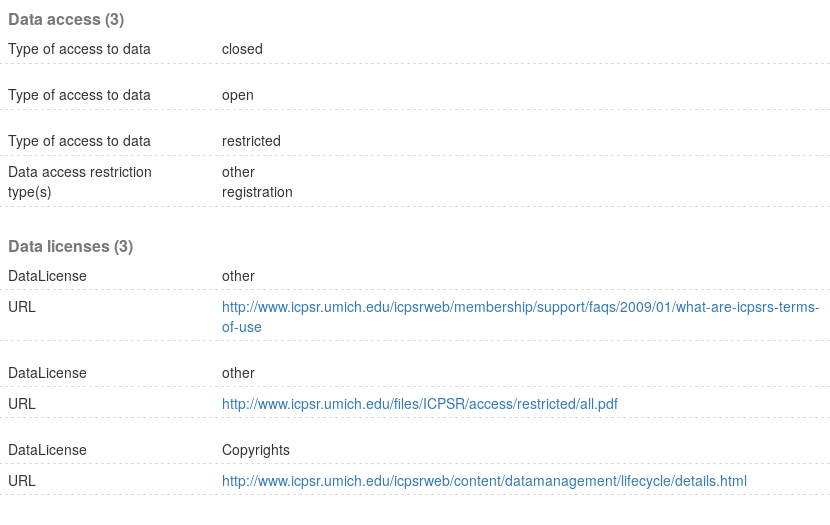
\includegraphics[width=1\textwidth]{\suppDir/re3data-org-icpsr-access-licenses-20181008.png}
	%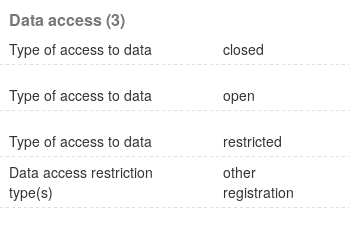
\includegraphics[width=0.4\textwidth]{re3data-org-icpsr-access-20181008.png}
\end{figure}
Thus, while re3data does contain entries of \textit{possible} licenses, we have no information on which one applies to the replication package above. Furthermore (not displayed here), there is no machine-readable information on persistence. While knowledgable data archivists and librarians, as well as many social scientists, ``know'' that ICPSR is a reputable archive with a long history and presumably a long future, this is not encoded anywhere where non-domain experts could ascertain it.

\paragraph{CoreTrustSeal}
We do not investigate whether this information is available  through CoreTrustSeal, for three reasons. First, searching again, as we did, through the website, neither of the search terms that the DataCite record provides yield findable results. Second, when we manually identify ICPSR on the website's map of institutions, we observe that ICPSR had a ``Data Seal of Approval'' (the predecessor to CoreTrustSeal), but that it expired in 2017, which may explain the lack of search results. Finally, the CoreTrustSeal certification is encapsulated in PDFs, and does not provide an API to search for attributes of a certified repository. While it may be feasible for a human to track down the relevant information, it is not scalable.
\FloatBarrier
\paragraph{Data publisher website}
\newcommand{\icpsrdate}{8 October 2018}
\begin{figure}
	\lstinputlisting[language=xml]{\suppDir/extract-webpage-20181008.xml}
	\caption{Use Case 1, Encoding of license in HTML of landing page}
	\label{fig:case1:rela}
\end{figure}
\begin{figure}
	\centering
	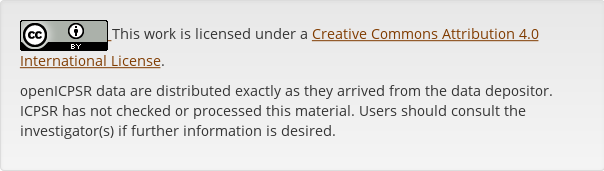
\includegraphics[width=0.5\linewidth]{\suppDir/../images/openicpsr-license-image.png}
	\caption{Use Case 1, license as displayed on website on \icpsrdate }
	\label{fig:case1:license}
\end{figure}
Finally, we attempt to obtain metadata   directly from the landing page indicated by the \ac{DOI}.%
\footnote{The query was run on \icpsrdate .}
The page offers five types of metadata: the in-page metadata in XML format, in-page metadata encoded as JSON-LD, a link to a OAI-PMH record, a link to a DDI 2.5 record, and a link to a DDI 3.1 record.
The webpage provides two instances of license information. The first instance is within the \texttt{rel} identifier within the \lstinline|a| link field (Figure~\ref{fig:case1:rela}) with an associated displayed  license badge (Figure~\ref{fig:case1:license}).
The second instance is encoded in the JSON-LD payload,
\begin{lstlisting}
"license":"https://creativecommons.org/licenses/by/4.0/deed.en_US"
\end{lstlisting}
Both provide the same information about the license.


\paragraph{Conclusion on Use Case 1}
We note that re3data did not provide additional information about  accessibility, even though ICPSR does provide data with more restrictive access rules, for instance, through secure cloud instances. Furthermore, no information is provided  about persistence. The openICPSR FAQ contain such information, but do so somewhat obliquely, and do not point to a policy. Browsing the website, one might encounter the ``\href{https://www.icpsr.umich.edu/icpsrweb/content/datamanagement/preservation/policies/index.html}{Digital Preservation Policies and Planning at ICPSR}'' \parencite{icpsr-preservation}, which  lays out the policies. 

We note that DataCite, while providing a means to communicate the license, did not do so at this time. DataCite does not provide a means to convey access rules or persistence, nor does it provide a means to point to specific policies on re3data. Re3data, in turn, lists three possible licenses, none of which apply in the present case, possibly because it lists information on the main ICPSR repository, and not on the associated but distinct openICPSR instance.

In this relatively straightforward case, we would need to query the user  about  which access policy applies to the particular dataset at hand. 

\section{Use Case 2: Restricted-access PSID}
The \ac{PSID} has published data for several decades, and is widely used (several thousand articles). Currently, researchers access the data by downloading them from the \ac{PSID} website, if the data is public-use. \ac{PSID} also provides some restricted access files, for instance with more detailed geocodes. Access procedures are described at \url{https://simba.isr.umich.edu/restricted/ProcessReq.aspx}. The \ac{PSID} has not assigned \ac{DOI} to any of its data products. Personal communication reveals that both public-use and restricted-access data are versioned internally, and that the data themselves contain a variable with the versioning information; there is, however, no metadata on the website listing the available past datasets, only the most current one. There is no explicit retention information on the website.

In this scenario, 
\begin{itemize}
	\item CrossRef or DataCite offer no information on the data
	\item While there is a re3data page at \url{https://www.re3data.org/repository/r3d100011131} \parencite{Re3data-psid}, it does not provide information on the restricted access conditions
	\item the product page offers some unstructured information
\end{itemize}
We also note that even if re3data had the correct access policy for 2018, it is difficult to obtain information on past access policies. The \ac{PSID} used to provide restricted-access data via shipment of CDs to researchers, who would put the data on computers that were not connected to networks, secured in a locked room. Authors are still publishing articles today that rely on data obtained through the outdated access mode. 

\section{Use Case 3: Restricted access at the U.S. Census Bureau}

The \ac{LBD} data \parencite{MirandaJarmin2002,LBD}  at the U.S. Census Bureau is one of the most requested datasets in the \ac{FSRDC} network. Access procedures are described at various locations, including \urlcite{https://www.census.gov/ces/rdcresearch/index.html}{here} and \urlcite{https://www.census.gov/ces/rdcresearch/howtoapply.html}{here}. The LBD data, as most business data at the U.S. Census Bureau, contain \ac{FTI}; however, this is not noted on the product description page. In contrast to many person or household data, which are archived at the National Archives as per a published Records Schedule, the business data are not sent to the National Archives, due to the presence of said \ac{FTI}. It is quite difficult to find information on this. In fact, the Center for Economic Studies is the official archiver, and maintains these files in perpetuity. The Census Bureau has not assigned \ac{DOI} to any of its data assets as of 2018.


In this scenario, 
\begin{itemize}
	\item CrossRef or DataCite offer no information on the data
	\item While there is a re3data page at \url{https://www.re3data.org/repository/r3d100010200} \parencite{Re3data-uscb}, it does not provide any information on the \ac{FSRDC} (the entry has several other issues as well, regarding license information, but those are not relevant here)
	\item the product page offers no structured information, and policy information is scattered throughout the website.
\end{itemize}



%\bibliographystyle{chicagoa}
%\bibliography{references.bib}
\printbibliography[title=References Cited]

\end{document}
